\subsection{Ticket Issuance}
\label{sec:tickets:issuance}

A ticket can be issued once two nodes have established a payment channel with each other. By definition this means at least one of them has staked HOPR tokens. A ticket is issued by a node for the next downstream relay node along the path. In the following, we describe this process between the sender $A$ and the first downstream node $B$ but the same process applies for the ticket that is issued by $B$ for $C$ and following nodes.

The ticket issuer $A$ (who could also be the packet creator) sets a winning probability and relay fee to use and sets the amount to: $$\sigma=\dfrac{L\times F}{P_w}$$ where $\sigma$ is the amount of HOPR tokens set in the ticket, $L$ is the path length, $F$ is the relay fee, and $P_w$ is the ticket's winning probability. These are currently static values which apply network wide.

$A$ issues a ticket for the next downstream node. The challenge is given together with the routing information by the packet. $A$ does not know whether the ticket is a winner or not.

$A$ sets the content of the ticket to: $$t=(R,\sigma,P_w,\alpha,I,T_c,\zeta),$$ where $t$ has the following components, in addition to those already defined above:

\begin{itemize}
    \item
          \textbf{Recipient's Ethereum address $R$}: a unique identifier derived from the ticket recipient's public key.
    \item
          \textbf{Ticket epoch $\alpha$}: used as a mechanism to prevent cheating by turning non-winning tickets into winning ones. This is done by increasing the value of $\alpha$ whenever a node resets a commitment, which helps keep track of updates to the on-chain commitments and invalidates tickets from earlier epochs.
    \item
          \textbf{Ticket index $I$}: set by the ticket issuer and increases with every issued ticket. The recipient verifies that the index increases with every packet and drops any packets where this is not the case. Redeeming a ticket with index $n$ invalidates all tickets with index $I<n$, hence the relayer has a strong incentive to not accept tickets with an unchanged index.
    \item
          \textbf{Ticket challenge $T_c$}: set by the ticket issuer and used to check whether a ticket is redeemable before the packet is been relayed. If it is not redeemable, the packet is dropped.
    \item
          \textbf{Channel epoch $\zeta$}: used to give each incarnation of the payment channel a new identifier such that tickets issued for previous instances of the channel become invalid once a channel is reopened ($\alpha$'s count restarts again). This is due to the fact that $\zeta$ increments whenever a closed channel is (re)opened.
\end{itemize}

$A$ then signs the ticket with its private key and sends $T = (t, Sig_I(t))$ to the recipient together with a mixnet packet.
\begin{comment}


\\\textbf{ChainId $c_{Id}$:} The channel identifier which is defined by the ticket issuer in order to determine which channel will be used between issuer and next downstream node. For example, tickets that are valid on xDAI are not valid on Ethereum.
\\\textbf{Tag $\tau$} is given as a constant and depends on the utilized blockchain. It is used to distinguish HOPR tickets from others with the same structure that are meant for different payment channels and invalidates their usage in HOPR.
\\\textbf{Version $V$} is given as a constant and depends on the utilized blockchain. It is used to invalidate tickets that were issued for previous versions of HOPR from being used in future iterations of the protocol.

\end{comment}

\begin{figure}[H]
    \centering
    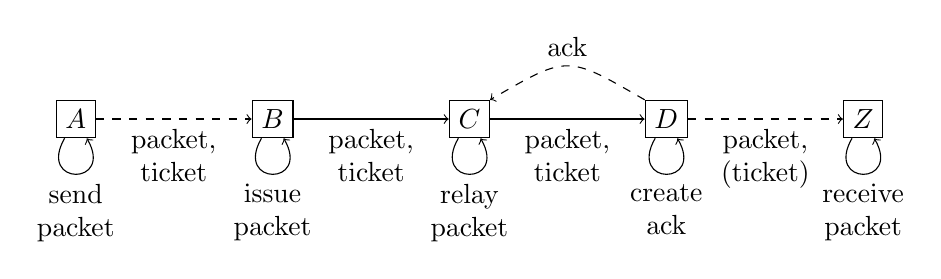
\begin{tikzpicture}[auto]
        \draw (0,0) node (a) [rectangle,draw] {$A$};
        \draw (2.5,0) node (b) [rectangle,draw] {$B$};
        \draw (5,0) node (c) [rectangle,draw] {$C$};
        \draw (7.5,0) node (d) [rectangle,draw] {$D$};
        \draw (10,0) node (z) [rectangle,draw] {$Z$};

        \draw [->,draw,dashed] (a.east) to node [align=center,below] {packet,\\ticket} (b.west);
        \draw [->,draw] (b.east) to node [align=center,below] {packet,\\ticket} (c.west);
        \draw [->,draw] (c.east) to node [align=center,below] {packet,\\ticket} (d.west);
        \draw [->,draw,dashed] (d.east) to node [align=center,below] {packet,\\(ticket)}  (z.west);

        \path[->] (a) edge [out=-120,in=-60,distance=2em,below] node [align=center] {send\\packet}  (a);    % \draw 
        \path[->] (b) edge [out=-120,in=-60,distance=2em,below] node [align=center] {issue\\packet}  (b);    % \draw 
        \path[->] (c) edge [out=-120,in=-60,distance=2em,below] node [align=center] {relay\\packet}  (c);    % \draw 
        \path[->] (d) edge [out=-120,in=-60,distance=2em,below] node [align=center] {create\\ack}  (d);    % \draw 
        \path[->] (z) edge [out=-120,in=-60,distance=2em,below] node [align=center] {receive\\packet}  (z);    % \draw 

        \path[->,draw,looseness=1.5,dashed,bend right] (d.north west) to [above] node {ack} (c.north east);
    \end{tikzpicture}    \caption{Ticket workflow}
    \label{fig:Ticket worklow}
\end{figure}